\documentclass{article}
\usepackage[utf8]{inputenc}
\usepackage[papersize={8.5in,11in},margin=0.8in]{geometry}
\usepackage{xcolor}
\usepackage{color, colortbl}
\usepackage{graphicx}
\usepackage{tikz}
\usepackage{amssymb}
\usetikzlibrary{positioning}


\title{MATH 505 HW 5}
\author{John Caruthers}
\date\today

\begin{document}
\maketitle

\textbf{Section 2.3}

\begin{itemize}
    \item[1.] Consider the following game of "What's My Rule?"  When Al said 3, I said 8.  When Bo said 5, I said 24.  When Carol said 2, I said 3.  When Diane said 1, I said 0.
    
    (a) Describe this "rule" as a set of ordered pairs.\\
    \hspace*{0.5cm}{\color{blue} $\{(3,8),(5,24),(2,3),(1,0)\}$}
    
    (b) If Eddie says 4, what do you think I will say?\\
    \hspace*{0.5cm}{\color{blue} 15}
    
    (c) What's my rule? In other words, write a rule in words for the game.\\
    \hspace*{0.5cm}{\color{blue} The rule is to take the input number, square it then subtract 1.}
    
    (d) Use function notation to describe this rule.\\
    \hspace*{0.5cm}{\color{blue} $f(x)=x^2-1$}
    
    \item[5.] Which of the following arrow diagrams represent a function?\\
    {\color{blue} A, B and D represents a function.}
    
    
%%    \begin{tikzpicture}
%%   [
%%    mydot/.style={circle,fill,inner sep=2pt},
%%   >=latex
%%    ]
%%    \node[mydot,label={left:1}] (a1) {};
%%    \node[mydot,below=0.3cm of a1,label={left:2}] (a2) {};
%%    \node[mydot,below=0.3cm of a2,label={left:3}] (a3) {};
%%    \node[mydot,below=0.3cm of a3,label={left:4}] (a4) {};
%%    \node[mydot,below=0.3cm of a4,label={left:5}] (a5) {};
%%
%%    \node[mydot,right=2cm of a1,label={right:1}] (b1) {};
%%    \node[mydot,below=0.3cm of b1,label={right:2}] (b2) {};
%%    \node[mydot,below=0.3cm of b2,label={right:3}] (b3) {};
%%    \node[mydot,below=0.3cm of b3,label={right:4}] (b4) {};
%%    \node[mydot,below=0.3cm of b4,label={right:5}] (b5) {};
%%
%%    \path[->] (a1) edge (b3);
%%    \path[->] (a2) edge (b4);
%%    \path[->] (a4) edge (b5);
%%    \path[->] (a5) edge (b1);
%%    \end{tikzpicture}
    
    
    \item[6.] Represent each of the relations in Exercise 5 as a set of ordered pairs.
    
    (a) {\color{blue} $\{(1,1),(2,1),(3,5),(4,4),(5,4)\}$}
    
    (b) {\color{blue} $\{(1,4),(2,5),(3,2),(4,4),(5,1)\}$}
    
    (c) {\color{blue} $\{(1,4),(2,1),(3,3),(4,2),(5,4)\}$}
    
    (d) {\color{blue} $\{(1,3),(2,4),(4,5),(5,1)\}$}
    
    \item[7.] For each of the relations in Exercise 5:
    
    (a) Give the domain and range for each.\\
    \hspace*{0.5cm}(a) {\color{blue} Domain: $\{1,2,3,4,5\}$, Range: $\{1,4,5\}$}
    
    \hspace*{0.5cm}(b) {\color{blue} Domain: $\{1,2,3,4,5\}$, Range: $\{1,2,4,5\}$}
    
    \hspace*{0.5cm}(c) {\color{blue} Domain: $\{1,2,3,4,5\}$, Range: $\{1,2,3,4,5\}$}
    
    \hspace*{0.5cm}(d) {\color{blue} Domain: $\{1,2,4,5\}$, Range: $\{1,3,4,5\}$}
    
    (b) Which functions are one-to-one?\\
    \hspace*{0.5cm}{\color{blue} Only D is one to one. }
    
    (c) Which are onto the set $\{1, 2, 3, 4, 5\}$?\\
    \hspace*{0.5cm}{\color{blue} Only C is onto the set $\{1, 2, 3, 4, 5\}$ because every element is an output of some input.}
    
    
    \item[8.] Draw an arrow diagram to represent each of the following functions on the set $\{1, 2, 3, 4, 5\}$.
    
    (a) $f(x)=6-x$\\
    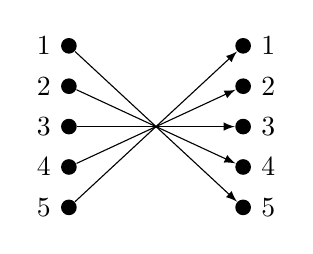
\begin{tikzpicture}
    [
    mydot/.style={circle,fill,inner sep=2pt},
    >=latex
    ]
    \node[mydot,label={left:1}] (a1) {};
    \node[mydot,below=0.3cm of a1,label={left:2}] (a2) {};
    \node[mydot,below=0.3cm of a2,label={left:3}] (a3) {};
    \node[mydot,below=0.3cm of a3,label={left:4}] (a4) {};
    \node[mydot,below=0.3cm of a4,label={left:5}] (a5) {};

    \node[mydot,right=2cm of a1,label={right:1}] (b1) {};
    \node[mydot,below=0.3cm of b1,label={right:2}] (b2) {};
    \node[mydot,below=0.3cm of b2,label={right:3}] (b3) {};
    \node[mydot,below=0.3cm of b3,label={right:4}] (b4) {};
    \node[mydot,below=0.3cm of b4,label={right:5}] (b5) {};

    \path[->] (a1) edge (b5);
    \path[->] (a2) edge (b4);
    \path[->] (a3) edge (b3);
    \path[->] (a4) edge (b2);
    \path[->] (a5) edge (b1);
    \end{tikzpicture}
    
    (b) $f(x)=(x-3)^2$\\
    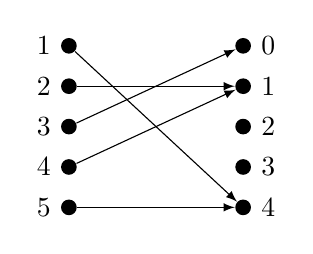
\begin{tikzpicture}
    [
    mydot/.style={circle,fill,inner sep=2pt},
    >=latex
    ]
    \node[mydot,label={left:1}] (a1) {};
    \node[mydot,below=0.3cm of a1,label={left:2}] (a2) {};
    \node[mydot,below=0.3cm of a2,label={left:3}] (a3) {};
    \node[mydot,below=0.3cm of a3,label={left:4}] (a4) {};
    \node[mydot,below=0.3cm of a4,label={left:5}] (a5) {};

    \node[mydot,right=2cm of a1,label={right:0}] (b0) {};
    \node[mydot,below=0.3cm of b0,label={right:1}] (b1) {};
    \node[mydot,below=0.3cm of b1,label={right:2}] (b2) {};
    \node[mydot,below=0.3cm of b2,label={right:3}] (b3) {};
    \node[mydot,below=0.3cm of b3,label={right:4}] (b4) {};

    \path[->] (a1) edge (b4);
    \path[->] (a2) edge (b1);
    \path[->] (a3) edge (b0);
    \path[->] (a4) edge (b1);
    \path[->] (a5) edge (b4);
    \end{tikzpicture}
    
    (c) $f(x)=2x-3$\\
    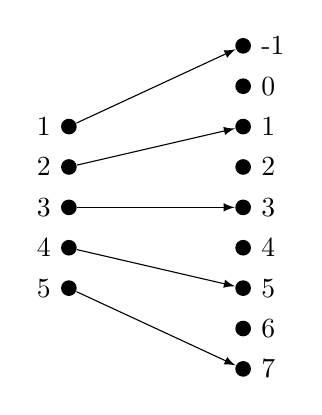
\begin{tikzpicture}
    [
    mydot/.style={circle,fill,inner sep=2pt},
    >=latex
    ]
    \node[mydot,label={left:1}] (a1) {};
    \node[mydot,below=0.3cm of a1,label={left:2}] (a2) {};
    \node[mydot,below=0.3cm of a2,label={left:3}] (a3) {};
    \node[mydot,below=0.3cm of a3,label={left:4}] (a4) {};
    \node[mydot,below=0.3cm of a4,label={left:5}] (a5) {};

    \node[mydot,right=2cm of a1,label={right:1}] (b1) {};
    \node[mydot,above=0.3cm of b1,label={right:0}] (b0) {};
    \node[mydot,above=0.3cm of b0,label={right:-1}] (b11) {};
    \node[mydot,below=0.3cm of b1,label={right:2}] (b2) {};
    \node[mydot,below=0.3cm of b2,label={right:3}] (b3) {};
    \node[mydot,below=0.3cm of b3,label={right:4}] (b4) {};
    \node[mydot,below=0.3cm of b4,label={right:5}] (b5) {};
    \node[mydot,below=0.3cm of b5,label={right:6}] (b6) {};
    \node[mydot,below=0.3cm of b6,label={right:7}] (b7) {};

    \path[->] (a1) edge (b11);
    \path[->] (a2) edge (b1);
    \path[->] (a3) edge (b3);
    \path[->] (a4) edge (b5);
    \path[->] (a5) edge (b7);
    \end{tikzpicture}

\end{itemize}

\textbf{Section 2.4}

\begin{itemize}
    \item[1.] Write down the first five terms of the sequence whose general term is given by:
    
    (a) $a_n=n+4$
    
    {\color{blue}$5,6,7,8,9,...$}
    
    (c) $a_n=\frac{1}{n}$
    
    {\color{blue}$\{1,\frac{1}{2},\frac{1}{3},\frac{1}{4},\frac{1}{5}\}$}
    
    (e) $a_n=n^2+1$\\
    {\color{blue}$2,5,10,17,26,...$}
    
    (g) $a_n=2\cdot(-1)^n$\\
    {\color{blue}$-2,2,-2,2,-2,...$}
    
    (i) $a_n=5\cdot2^n$\\
    {\color{blue}$10,20,40,80,160,...$}
    
    \item[3.] Describe a pattern in words, and then find the next three terms for each of the following:
    
    (a) $3, 7, 11, 15, 19, ...$
    
    {\color{blue} $a_1$ is 3 and every number after is the previous number plus $4$. The next three are: $23, 27, 31$}
    
    (c) $8, 2, -4, -10, -16, ...$
    
    {\color{blue} $a_1$ is 8 and every number after is the previous number minus 6. The next three are: $-22,-28,-34$}
    
    (e) $\frac{1}{3}, \frac{1}{9}, \frac{1}{27}, \frac{1}{81}, \frac{1}{243}, ...$
    
    {\color{blue} $a_1$ is $\frac{1}{3}$, and every number after is the previous number multiplied by $\frac{1}{3}$. The next three are: $\frac{1}{729}, \frac{1}{2187}, \frac{1}{6561}$.}
    
    (g) $1, 6, 5, 10, 9, ...$
    
    {\color{blue} $a_1$ is 1 and the next number is the previous number plus 5 if the previous number is odd, or the next number is the previous number minus 1 if the previous number is even. The next three are: $14, 13, 18$.}
    
    (i) $1, 3, 6, 10, 15, ...$
    
    {\color{blue} $a_1$ is 1 and every number after is the previous number plus the $n$ value of the number to be calculated. The next three are: $21, 28, 36$. }
    
    \newpage
    
    \item[5.] For each of the following sequences, determine whether the sequence could be arithmetic, geometric, or neither.  If it is arithmetic, give the common difference \emph{d}. If it is geometric, give the common ratio, \emph{r}.
    
    (a) 1, 0, 1, 0, 1, ... 
    
    {\color{blue} It seems to be neither arithmetic or geometric, however we could set $a_n=n\bmod(2)$, to get the same sequence.}
    
    (b) 9, 7, 5, 3, 1, ...
    
    {\color{blue} Arithmetic, $d=-2$.}
    
    (c) 1, -1, 1, -1, 1, ...
    
    {\color{blue}Geometric, $r=-1$.}
    
    (d) 4, 20, 100, 500, 2500, ...
    
    {\color{blue}Geometric, $r=5$.}
    
    (e) 2, -4, 6, -8, 10, ...
    
    {\color{blue}Neither}
    
    \item[18.] Suppose a sequence has the first term 2 and the third term 18.
    
    (a) If the sequence is arithmetic, find the common difference \emph{d}, and list the first five terms of the sequence.
    
    {\color{blue} $d=8$, and the first five terms are: $2,10,18,26,34,...$.}
    
    (b) If the sequence is geometric, find two possible values for the common ration \emph{r}, and list the first five terms of the geometric sequence in each case. 
    
    {\color{blue} $r=3$; the first five terms are: $2,6,18,54,162$, and $r=-3$; the first five terms are: $2,-6,18,-54,162,...$.} 
    
\end{itemize}

\textbf{Section 2.5}

\begin{itemize}
    \item[Exp 4.] In computer science, a \emph{bit string}  is a sequence of zeros and ones.
    
    (a) List the bit strings of length one.
    
    {\color{blue} 0, 1}
    
    (b) List the bit strings of length two that contain no two consecutive 1's.
    
    {\color{blue} 00, 01, 10}
    
    (c) List the bit strings of length three that contain no two consecutive 1's.
    
    {\color{blue} 000, 001, 010, 100, 101}
    
    (d) List the bit strings of length four that contain no two consecutive 1's.
    
    {\color{blue} 0000, 0001, 0010, 0100, 1000, 0101, 1010, 1001}
    
    (e) What do you notice about the number of bit strings in your answers? Answer by completing the following conjecture: \textbf{Conjecture:} The number of bit strings of length $n$ that contain no two consecutive 1's is {\color{blue} $f_n=f_{n-1}+f_{n-2}$}, where $f_n$ denoted the $n$th term of the Fibonacci sequence: $1, 1, 2, 3, 5, 8, ...$
    
    \item[1.] Write down the first five terms of each of the following recursive sequences:
    
    (a) $a_1=12$ and $a_n=a_{n-1}-2$ for $n\geq2$
    
    {\color{blue}$12,10,8,6,4,...$}
    
    (b) $a_1=5$ and $a_n=2a_{n-1}$ for $n\geq2$
    
    {\color{blue}$5,10,20,40,80,...$}
    
    \item[5.] Write down the first five terms of each of the following sequences:
    
    (a) $a_1=1$ and $a_n=n\cdot a_{n-1}$ for $n\geq2$
    
    {\color{blue}$1,2,6,24,120,...$}
    
    (b) $a_1=1$ and $a_n=n\cdot a_{n-1}+1$ for $n\geq2$
    
    {\color{blue}$1,3,10,41,206,...$}
    
    \item[8.] Suppose a sequence had the recurrence relation $a_n=a_{n-1}+a_{n-2}$ for $n\geq3$. Write down the first ten terms of the sequence if the initial terms are:
    
    (a) $a_1=1$ and $a_2=3$
    
    {\color{blue}$4,7,11,18,29,47,76,123,..$}
    
    (b) $a_1=3$ and $a_2=1$
    
    {\color{blue}$4,5,9,14,23,37,60,97,...$}
    
    (c) $a_1=2$ and $a_2=-1$
    
    {\color{blue}$1,0,1,1,2,3,5,8,...$}
    
    (d) $a_1=5$ and $a_2=-3$
    
    {\color{blue}$2,-1,1,0,1,1,2,3,...$}
    
    \item[9.] 
    
    (a) Write down the first five terms of the sequence defined by $a_1=1, a_2=2,$ and $a_n=(n-1)(a_{n-1}+a_{n-2})$ for $n\geq3$.
    
    {\color{blue} $1,2,6,24,120,...$}
    
    (b) Write down the first five terms of the sequence defined by $a_1=1$ and $a_n=n\cdot a_{n-1}$ for $n\geq2$.
    
    {\color{blue} $1,2,6,24,120,...$}
    
    (c) What do you notice about the two sequences in part (a) and (b)?
    
    {\color{blue} These two sequences are equal.}
\end{itemize}

\end{document}
